\section{Cipher Abjad-Majemuk (\textit{Polyalphabetic})}
\label{sec:abjad-majemuk}

Untuk mengatasi kelemahan analisis frekuensi, dikembangkanlah
\textit{polyalphabetic cipher}, yaitu cipher yang memakai beberapa abjad
substitusi sekaligus. Pada cipher jenis ini, satu huruf plainteks dapat
dienkripsi menjadi huruf cipherteks yang berbeda-beda tergantung pada
posisinya di dalam pesan. Akibatnya, puncak frekuensi huruf plainteks tidak
lagi tampak sebagai puncak pada cipherteks, sehingga langkah pertama analisis
frekuensi kehilangan pijakannya.

Rumusan umumnya adalah sebagai berikut. Misalkan kunci $K = k_1 k_2 \cdots
k_m$ berpanjang $m$, dan plainteks $P = p_1 p_2 \cdots p_m p_{m+1} \cdots$.
Cipherteksnya dibentuk dengan memakai huruf kunci secara bergiliran:
\[
C = E_k(P) = f_{k_1}(p_1)\, f_{k_2}(p_2) \cdots f_{k_m}(p_m)\,
f_{k_1}(p_{m+1}) \cdots,
\]
dengan setiap $f_{k_i}$ adalah sebuah abjad substitusi yang berbeda.
Perhatikan bahwa bila $m = 1$, rumus itu menyusut kembali menjadi cipher
abjad-tunggal. Jadi cipher abjad-majemuk bukanlah jenis cipher yang sama sekali
baru, melainkan \emph{perulangan} cipher abjad-tunggal dengan kunci yang
berganti-ganti \citep{stinson2018}.

\subsection{Vigen\`ere Cipher}
\label{sec:vigenere}

Vigen\`ere cipher menggunakan kata kunci yang diulang secara periodik
sepanjang pesan. Jika panjang kunci adalah $m$, maka huruf ke-$j$ dienkripsi
menggunakan pergeseran yang ditentukan oleh huruf kunci ke-$(j \bmod m)$.
Karena pergeseran berganti setiap huruf, Vigen\`ere cipher secara efektif
adalah rangkaian Caesar cipher dengan kunci yang berbeda-beda, dan itulah
sebabnya cipher ini disebut juga cipher abjad-majemuk.

\textbf{Mekanisme kerja.} Enkripsi dapat dilakukan dengan menelusuri
\textit{Vigen\`ere square} --- tabel bujursangkar berisi 26 baris alfabet yang
tiap barisnya digeser satu posisi dari baris di atasnya
(Gambar~\ref{fig:vigenere-square}) --- atau secara matematis dengan rumus
\begin{equation}
    c_j = (p_j + k_i) \bmod 26,
    \qquad
    p_j = (c_j - k_i) \bmod 26,
    \label{eq:vigenere}
\end{equation}
dengan $k_i$ adalah huruf kunci yang berlaku pada posisi tersebut. Baris ke-0
pada Vigen\`ere square adalah alfabet tanpa pergeseran, baris ke-1 bergeser
satu posisi, dan seterusnya sampai baris ke-25 \citep{stinson2018}.

\begin{figure}[htbp]
    \centering
    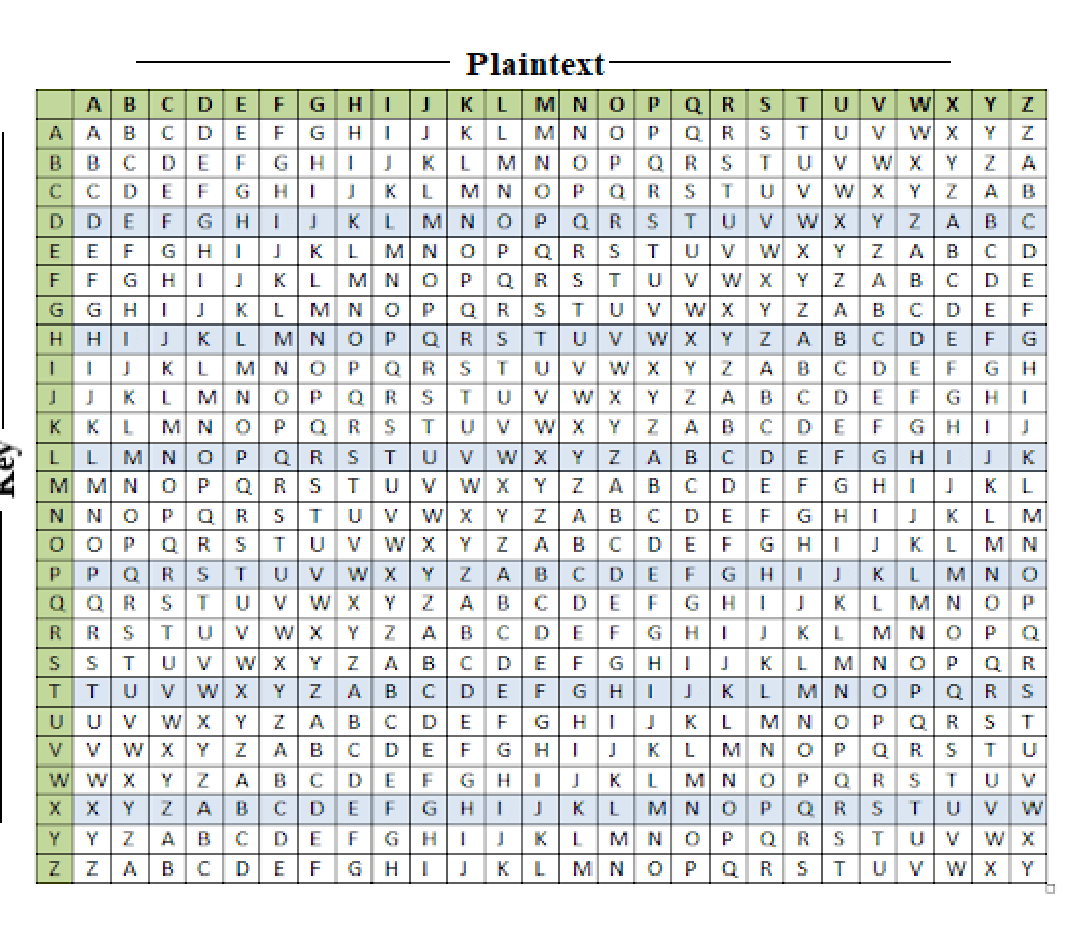
\includegraphics[width=0.85\linewidth, height=0.6\textheight, keepaspectratio]{figures/vigenere-square.png}
    \caption{\textit{Vigen\`ere square}: baris ke-$k$ berisi alfabet yang digeser $k$ posisi. Setiap huruf plainteks dienkripsi memakai baris yang ditentukan oleh huruf kuncinya}
    \label{fig:vigenere-square}
    \sumber{Munir, \textit{IF4020 Kriptografi}, ITB.}
\end{figure}

\textbf{Contoh terhitung.} Misalkan kunci yang dipakai adalah \code{soreang}
dengan nilai $(18, 14, 17, 4, 0, 13, 6)$ dan plainteksnya
\code{terimapesanangulaikambing} yang berisi 25 huruf. Kunci diulang sehingga
panjangnya menyamai plainteks, yaitu menjadi
\code{soreangsoreangsoreangsore}. Untuk tiga huruf pertama:
\[
\begin{array}{cccc}
P & t = 19 & e = 4 & r = 17\\
K & s = 18 & o = 14 & r = 17\\
\hline
C & (19+18)_{26} = 11 = L & (4+14)_{26} = 18 = S & (17+17)_{26} = 8 = I
\end{array}
\]
Meneruskan cara yang sama untuk seluruh 25 huruf menghasilkan cipherteks
\begin{center}
\texttt{LSIMMNVWGRRAAMMZRMKNSTWEK}.
\end{center}
Dekripsi mengembalikannya melalui $p_j = (c_j - k_i) \bmod 26$; sebagai uji,
$L = 11$ dikurangi $s = 18$ memberikan $-7 \bmod 26 = 19 = t$, yaitu huruf
plainteks yang benar.

\textbf{Karakteristik yang penting.} Pada contoh di atas, huruf plainteks
\code{t} bisa menjadi \code{L} (posisi 1 dengan kunci $s$) maupun \code{H}
(posisi lain dengan kunci yang berbeda). Sebaliknya, huruf cipherteks
\code{V} dapat berasal dari \code{H}, \code{I}, atau \code{X}. Pemetaan yang
berubah-ubah inilah yang membuat distribusi frekuensi huruf pada cipherteks
cenderung lebih seragam (\textit{flat}) dibandingkan monoalphabetic cipher,
sehingga cipher ini jauh lebih tahan terhadap analisis frekuensi sederhana
\citep{stallings2017}.

\subsubsection{Extended Vigen\`ere Cipher}

Alfabet Vigen\`ere tidak harus 26 huruf. Untuk mengenkripsi berkas biner atau
teks yang memuat angka dan tanda baca, dipakai \textbf{Extended Vigen\`ere
Cipher} dengan alfabet 256 karakter ASCII:
\[
c_j = (p_j + k_i) \bmod 256,
\qquad
p_j = (c_j - k_i) \bmod 256.
\]
Perluasan ini berguna untuk mengenkripsi berkas apa pun, bukan hanya teks
alfabet. Namun perhatikan bahwa perluasan alfabet \emph{tidak} menambah
kekuatan terhadap metode Kasiski, karena panjang kunci dan sifat
pengulangannya tidak berubah; yang berubah hanya ukuran alfabet.

\subsubsection{Sejarah Vigen\`ere Cipher}

Meskipun namanya diambil dari Blaise de Vigen\`ere (1523--1596), seorang
diplomat dan kriptografer Prancis pada masa Dinasti Valois, cipher
abjad-majemuk sebenarnya sudah diperkenalkan oleh Leon Battista Alberti pada
1467. Vigen\`ere mempublikasikan versinya yang lebih sederhana pada 1562
melalui karyanya \textit{Traict\'e des chiffres}, dan karena itulah namanya
melekat pada cipher ini. Selama berabad-abad Vigen\`ere cipher dianggap
\emph{le chiffre ind\'echiffrable} --- ``cipher yang tidak dapat dipecahkan''
--- sampai Charles Babbage berhasil memecahkannya pada pertengahan abad ke-19
dan Friedrich Kasiski mempublikasikan metode pemecahan yang sistematis pada
1863 \citep{stinson2018}. Potret Blaise de Vigen\`ere diperlihatkan pada
Gambar~\ref{fig:blaise-de-vigenere}.

\begin{figure}[htbp]
    \centering
    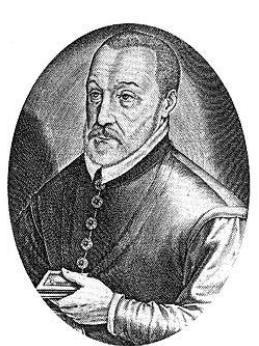
\includegraphics[width=0.22\linewidth, height=0.35\textheight, keepaspectratio]{figures/blaise-de-vigenere.png}
    \caption{Blaise de Vigen\`ere (1523--1596), diplomat dan kriptografer Prancis yang namanya dilekatkan pada cipher abjad-majemuk}
    \label{fig:blaise-de-vigenere}
    \sumber{Munir, \textit{IF4020 Kriptografi}, ITB.}
\end{figure}

\subsection{Kriptanalisis Vigen\`ere: Metode Kasiski}
\label{sec:kasiski}

Meskipun lebih kuat, Vigen\`ere cipher tetap dapat dipecahkan jika pesan cukup
panjang. Friedrich Kasiski (1863) menemukan bahwa jika sebuah kata di dalam
plainteks muncul berulang kali dan kebetulan berada pada posisi yang jaraknya
merupakan kelipatan panjang kunci, maka kedua kemunculan itu akan menghasilkan
kriptogram --- rangkaian huruf cipherteks --- yang sama. Pengamatan inilah
yang membuka jalan pemecahan \citep{kasiski1863,stinson2018}.

\begin{figure}[htbp]
    \centering
    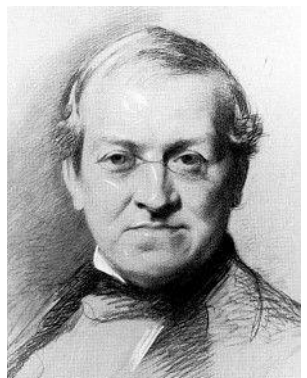
\includegraphics[width=0.25\linewidth, height=0.35\textheight, keepaspectratio]{figures/friedrich-kasiski.png}
    \caption{Friedrich Wilhelm Kasiski (1805--1881), perwira Prusia yang pada 1863 menjadi orang pertama yang memecahkan Vigen\`ere cipher secara sistematis}
    \label{fig:friedrich-kasiski}
    \sumber{Munir, \textit{IF4020 Kriptografi}, ITB.}
\end{figure}

Langkah-langkah metode Kasiski adalah sebagai berikut.
\begin{enumerate}
    \item Cari kriptogram yang berulang di dalam cipherteks.
    \item Hitung jarak antara kemunculan-kemunculan tersebut.
    \item Faktorkan setiap jarak; faktor-faktornya adalah calon panjang kunci.
          Irisan dari seluruh himpunan faktor memberikan estimasi panjang kunci
          $m$.
    \item Setelah $m$ diketahui, bagi cipherteks menjadi $m$ kelompok menurut
          posisi modulo $m$. Setiap kelompok sekarang merupakan cipher
          abjad-tunggal yang dapat dipecahkan dengan analisis frekuensi.
\end{enumerate}
Perhatikan bahwa metode Kasiski tidak langsung mengungkap huruf-huruf kunci;
ia hanya mengungkap \emph{panjang} kunci. Setelah panjang kunci diketahui, sisa
pekerjaan baru dapat dilakukan.

Untuk melihat mengapa jarak itu penting, perhatikan contoh berikut. Plainteks
\code{cryptoisshortforcryptography} dienkripsi dengan kunci \code{abcd} yang
berpanjang 4. Kata \code{crypto} muncul dua kali, dan jarak antara kedua
kemunculan itu adalah 16 huruf. Karena 16 habis dibagi 4, kedua kemunculan
\code{crypto} menghasilkan kriptogram yang sama, yaitu \code{CSASTP}, dan
itulah yang memberi tahu penyerang bahwa panjang kunci kemungkinan 4.
Gambar~\ref{fig:kasiski-jarak16} memperlihatkan penandaan jarak tersebut.
Sebaliknya, bila plainteks yang sama dienkripsi dengan kunci \code{abcdef}
berpanjang 6, jarak 16 \emph{tidak} habis dibagi 6, sehingga kata \code{crypto}
tidak menghasilkan kriptogram yang sama dan tidak ada petunjuk yang muncul
dari kata itu.

\begin{figure}[htbp]
    \centering
    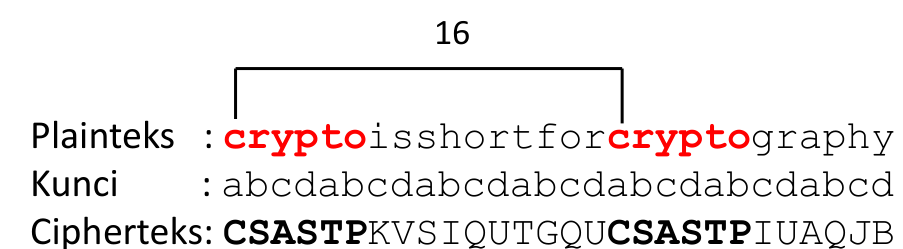
\includegraphics[width=0.9\linewidth, height=0.3\textheight, keepaspectratio]{figures/kasiski-jarak16.png}
    \caption{Jarak 16 huruf antara dua kemunculan kata \code{crypto}: karena 16 habis dibagi panjang kunci \code{abcd}, kedua kemunculan menghasilkan kriptogram yang sama}
    \label{fig:kasiski-jarak16}
    \sumber{Munir, \textit{IF4020 Kriptografi}, ITB.}
\end{figure}

\textbf{Contoh penerapan (jarak menentukan panjang kunci).} Misalkan di dalam
sebuah cipherteks ditemukan dua kriptogram yang berulang, yaitu
\code{DYDUXRMH} dan \code{NQD}. Jarak antara dua kemunculan \code{DYDUXRMH}
adalah 18, sehingga faktor-faktornya adalah $\{18, 9, 6, 3, 2\}$. Jarak antara
dua kemunculan \code{NQD} adalah 20, dengan faktor $\{20, 10, 5, 4, 2\}$.
Irisan kedua himpunan itu adalah $\{2\}$, sehingga panjang kunci paling
mungkin adalah 2.

\textbf{Contoh lengkap: menemukan kunci \code{SCRAM}.} Perhatikan cipherteks
yang memuat kriptogram \code{LJV} sebanyak enam kali. Jarak berturut-turut
antara kemunculannya adalah 15, 15, 15, 10, dan 10, sebagaimana diperlihatkan
pada Gambar~\ref{fig:kasiski-ljv}. Faktor dari 15 adalah $\{3, 5, 15\}$,
sedangkan faktor dari 10 adalah $\{2, 5, 10\}$. Satu-satunya nilai yang muncul
di kedua himpunan adalah 5, sehingga panjang kunci adalah 5.

Dengan panjang kunci 5, cipherteks dibagi menjadi lima kelompok menurut
posisinya, dan pada setiap kelompok dicari huruf yang paling sering muncul:
kelompok 1 didominasi \code{L}, kelompok 2 \code{J}, kelompok 3 \code{V},
kelompok 4 \code{N}, dan kelompok 5 \code{A}. Karena \code{LJV} adalah
kriptogram yang paling sering muncul, sangat mungkin rangkaian itu adalah
padanan trigram bahasa Inggris yang paling sering, yaitu \code{THE}. Dengan
pemetaan $\code{L} \rightarrow \code{T}$, $\code{J} \rightarrow \code{H}$, dan
$\code{V} \rightarrow \code{E}$, setiap huruf kunci dihitung sebagai
$K = (C - P) \bmod 26$:
\[
\begin{array}{cccccc}
\text{Kriptogram} & L=11 & J=9 & V=21 & N=13 & A=0\\
\text{Plainteks} & T=19 & H=7 & E=4 & N=13 & O=14\\
\hline
\text{Kunci} & 18 = S & 2 = C & 17 = R & 0 = A & 12 = M
\end{array}
\]
sehingga kuncinya adalah \code{SCRAM}. Gambar~\ref{fig:kasiski-scram}
memperlihatkan tabel pemetaan plainteks, cipherteks, dan kunci beserta nilai
numeriknya untuk kelima kelompok itu. Setelah kunci ditemukan, seluruh
cipherteks dapat didekripsi menjadi rangkaian sajak anak-anak:
\begin{quote}
\itshape
The bear went over the mountain yeah,\\
the dog went round the hydrant,\\
the cat into the highest spot he could find.
\end{quote}

\begin{figure}[htbp]
    \centering
    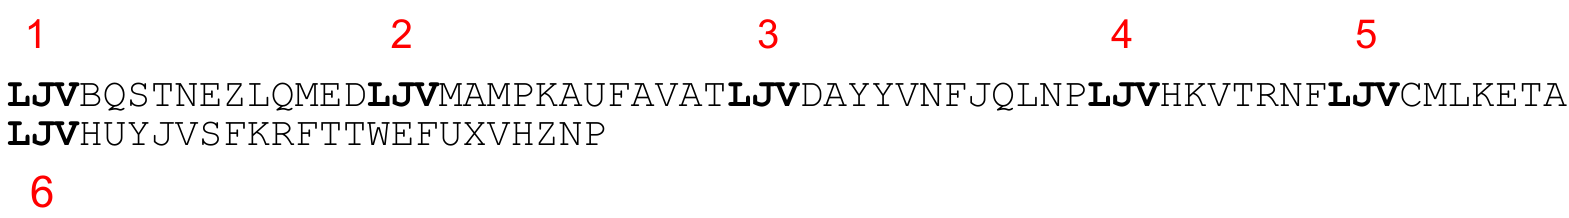
\includegraphics[width=0.95\linewidth, height=0.25\textheight, keepaspectratio]{figures/kasiski-ljv.png}
    \caption{Kriptogram \code{LJV} yang berulang enam kali pada cipherteks contoh; jarak antar kemunculannya adalah 15, 15, 15, 10, dan 10}
    \label{fig:kasiski-ljv}
    \sumber{Munir, \textit{IF4020 Kriptografi}, ITB.}
\end{figure}

\begin{figure}[htbp]
    \centering
    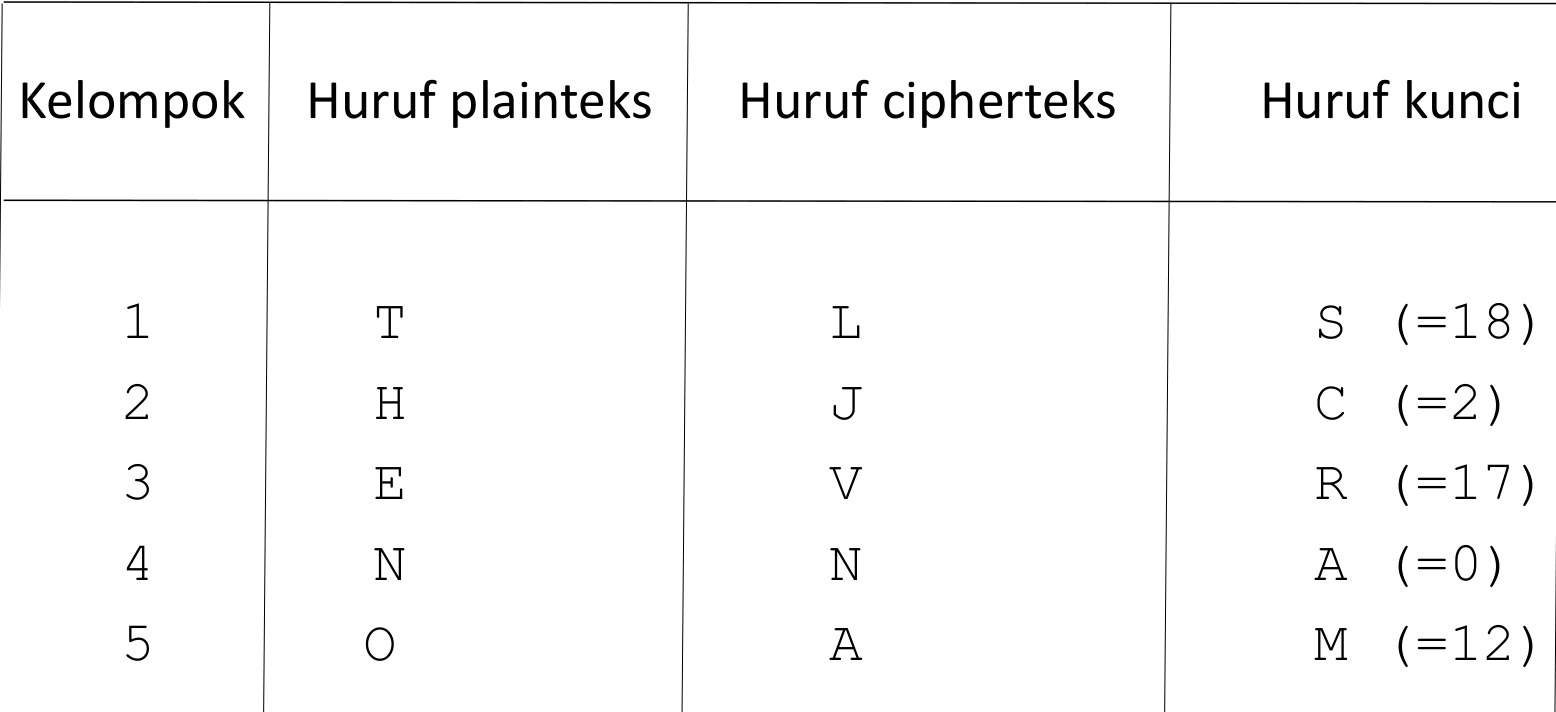
\includegraphics[width=0.95\linewidth, height=0.4\textheight, keepaspectratio]{figures/kasiski-scram.png}
    \caption{Tabel pemetaan plainteks, cipherteks, dan kunci beserta nilai numeriknya untuk kelima kelompok; huruf tersering tiap kelompok menghasilkan kunci \code{SCRAM}}
    \label{fig:kasiski-scram}
    \sumber{Munir, \textit{IF4020 Kriptografi}, ITB.}
\end{figure}

Perlu dicatat bahwa setelah panjang kunci $p$ diketahui, penyerang masih
mempunyai dua jalan. Jalan pertama adalah mencoba seluruh $26^p$ kemungkinan
kunci; jalan ini hanya praktis untuk $p$ yang sangat kecil. Jalan kedua adalah
analisis frekuensi pada masing-masing kelompok, yang jauh lebih efisien.
Tabel frekuensi acuan yang dipakai untuk keperluan itu --- sebagaimana
diperlihatkan pada Gambar~\ref{fig:tabel-frekuensi-huruf} --- adalah tabel
yang sama seperti pada analisis frekuensi cipher abjad-tunggal.

\begin{figure}[htbp]
    \centering
    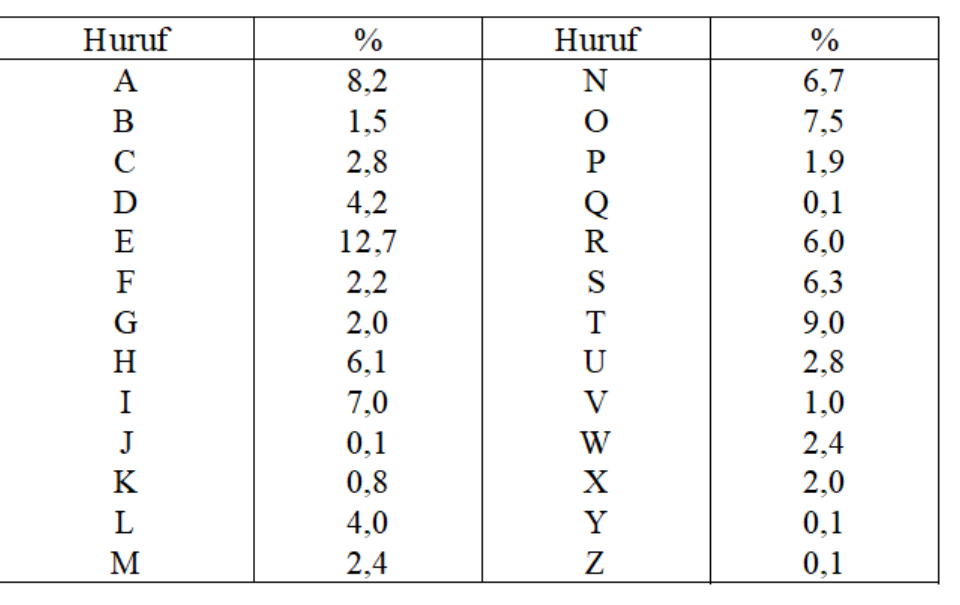
\includegraphics[width=0.85\linewidth, height=0.45\textheight, keepaspectratio]{figures/tabel-frekuensi-huruf.png}
    \caption{Frekuensi relatif kemunculan huruf alfabet bahasa Inggris; tabel acuan baku untuk kriptanalisis dengan analisis frekuensi}
    \label{fig:tabel-frekuensi-huruf}
    \sumber{Munir, \textit{IF4020 Kriptografi}, ITB.}
\end{figure}

\subsection{Varian Vigen\`ere}

Vigen\`ere cipher memiliki beberapa varian yang mencoba memperkuatnya dengan
mengubah cara kuncinya dibentuk. Perbedaan pokok ketiga varian itu
dirangkum pada Tabel~\ref{tab:varian-vigenere}, sedangkan aturan enkripsinya
tetap mengikuti Persamaan~\ref{eq:vigenere}.

\begin{table}[htbp]
\centering
\small
\begin{tabularx}{\linewidth}{@{}>{\raggedright\arraybackslash}p{3.1cm} >{\raggedright\arraybackslash}X >{\raggedright\arraybackslash}p{4.0cm}@{}}
\hline
\textbf{Varian} & \textbf{Cara membentuk kunci} & \textbf{Kelemahan} \\
\hline
Full Vigen\`ere & Setiap baris tabel adalah permutasi acak alfabet, bukan
pergeseran Caesar. Tabel harus dirahasiakan. & Keamanan bergantung pada
kerahasiaan tabel, bertentangan dengan Prinsip Kerckhoffs \\[4pt]
Auto-Key Vigen\`ere & Kunci awal disambung dengan plainteks itu sendiri,
sehingga panjang kunci menyamai pesan dan tidak ada pengulangan periodik &
Plainteks ikut terbaca pada bagian tabel kunci, sehingga kebocoran sebagian
plainteks membocorkan kunci \\[4pt]
Running-Key Vigen\`ere & Kunci diambil dari teks bermakna yang sangat panjang,
misalnya halaman buku atau naskah Pembukaan UUD 1945 & Keamanan bergantung pada
kerahasiaan teks kunci; bila teksnya dapat ditebak, kuncinya terbuka \\
\hline
\end{tabularx}
\caption{Perbandingan tiga varian Vigen\`ere cipher}
\label{tab:varian-vigenere}
\sumber{Data dari Munir, \textit{IF4020 Kriptografi}, ITB; tabel disusun dari uraian tersebut.}
\end{table}

\textbf{Full Vigen\`ere.} Pada varian ini, setiap baris tabel bukan lagi
alfabet yang digeser, melainkan permutasi acak dari seluruh alfabet. Karena
itu enkripsi tidak lagi merupakan penjumlahan modulo, dan tabelnya harus
disepakati serta dirahasiakan oleh kedua pihak. Secara praktis Full
Vigen\`ere menambah kerumitan, tetapi menyimpang dari prinsip bahwa keamanan
seharusnya terletak pada kunci, bukan pada algoritma yang dirahasiakan.

\textbf{Auto-Key Vigen\`ere.} Pada varian ini, pesan \code{negara penghasil
minyak mentah di dunia} dengan kunci awal \code{INDO} membentuk kunci
berpanjang penuh dengan menyambung kunci awal dan plainteksnya:
\begin{center}
\begin{tabular}{@{}l@{}}
\hline
Plainteks: \texttt{negarapenghasilminyakmentahdidunia}\\
Kunci: \texttt{INDONEGARAPENGHASILMINYAKMENTAHDID}\\
Cipherteks: \texttt{VRJOEEVEEGWEFOSMAVJMSZCNDMLQBDBQQD}\\
\hline
\end{tabular}
\end{center}
Perhatikan bahwa empat huruf pertama kunci adalah \code{INDO} yang dirahasiakan,
sedangkan sisanya adalah plainteks itu sendiri. Kelebihan varian ini adalah
tidak adanya pengulangan periodik, sehingga metode Kasiski tidak langsung
berlaku. Kelemahannya, sebagian tabel kunci justru memuat plainteks; bila
penyerang berhasil menebak isi pesan pada bagian awal, ia memperoleh kata
kunci pada bagian berikutnya.

\textbf{Running-Key Vigen\`ere.} Varian ini memakai teks bermakna yang sangat
panjang sebagai kunci, misalnya naskah Pembukaan UUD 1945. Untuk pesan
\code{negarapenghasilminyakmentahdidunia}, kuncinya adalah
\begin{center}
\texttt{KERAKYATANYANGDIPIMPINOLEHHIKMATPE}.
\end{center}
Selama teks kunci tidak dapat diduga dan tidak pernah diulang, Running-Key
Vigen\`ere cukup sulit dipecahkan. Namun bila penyerang mengenali teks
sumbernya --- dan naskah Pembukaan UUD 1945 adalah teks yang sangat mudah
dikenali di Indonesia --- maka kunci terbuka seluruhnya. Pelajaran dari ketiga
varian ini adalah sama: keamanan yang bergantung pada apa yang \emph{tidak}
diketahui penyerang, bukan pada kekuatan matematis, selalu rapuh
\citep{menezes1996}.
